\chapter{Optimization}

\label{chap:Optimization}

\section{Introduction}

As a system framework, REDHAWK is affected by system settings beyond the scope of REDHAWK. System optimization is sensitive to the set of applications that the system is intended to support. However, there are some simple settings that can apply to a wide set of applications. This chapter describes some of the effects of these generalized settings.

\section{Configuring omniORB}
\label{section:omniORBConfigurationPipes}

By default, omniORB configuration relies on the loopback interface of the operating system. While easy to use and manage, the loopback interface is not the fastest default transport that omniORB supports. omniORB also supports Linux Domain Sockets. Linux Domain Sockets are configured through the omniORB configuration file (/etc/omniORB.cfg).

The following steps explain how to configure Linux Domain Sockets.

\textbf{Note:} Root permissions are required to perform the following steps.

\begin{enumerate}
\item In the omiORB configuration file (/etc/omniORB.cfg), set the endpoints where the server is listening by adding the following lines to the endPoint section of the file:

\begin{terminalCode}
endPoint = giop:tcp:127.0.0.1:
         = giop:tcp:<computer IP address>:
         = giop:unix
\end{terminalCode}

\item Set the endpoints that are published in an object's \ac{ior} by adding the following lines to the endPointPublish section of the file:

\begin{terminalCode}
endPointPublish = all(addr)
\end{terminalCode}

After changing these settings, the name and event services must be reset, and their associated log files must be deleted. If the log files are not deleted,  they preserve \acp{ior} that are no longer valid.

\item Use the following commands to reset the name and event services and delete the associated files:

\begin{terminalCode}
# /etc/init.d/omniEvents stop
# /etc/init.d/omniNames stop
# rm -f /var/lib/omniEvents/*
# rm -f /var/omniNames/*
# /etc/init.d/omniNames start
# /etc/init.d/omniEvents start
\end{terminalCode}

\item To verify that Linux Domain Sockets are being used, go to /tmp, and verify that the omni-omni and omni-root directories exist. These two directories contain the files for the Linux Domain Sockets. Given that communications are now over file descriptors, verify that read permissions are open when communicating between objects owned by different users.

This change in the omniORB configuration greatly improves data transport rates.
\end{enumerate}

\section{Packet Transfer Size}

REDHAWK transfers data using \ac{bulkio}, which is an \ac{rpc} mechanism. The size of the data sequence that is passed on each of these calls has an effect on the data rate. The size of the transfer is not controlled by the REDHAWK runtime environment; instead, data producers can pass any arbitrary length less than \variable{giopMaxMsgSize}.

To demonstrate how throughput is affected by the configuration of omniORB and data transfer size, tests were performed on a system with the specifications shown in \link {Table}{table:ThroughputHostComputer}.

\ifpdf
%\\ \hline
\begin{longtable}{ |p{3.5cm}|p{3.5cm}|}
\caption{Computer Hosting Experiments} \label{table:ThroughputHostComputer} \\ \hline
\else
\begin{table}
\label{table:ThroughputHostComputer}
\begin{tabular}{ |p{3.5cm}|p{3.5cm}|}
\fi
  \textbf{Parameter} & \textbf{Value} \\ \hline
  Number of cores & 8 \\ \hline
  CPU clock speed & 3.40 GHz \\ \hline
  Cache size & 8192 kB \\ \hline
\ifpdf
\end{longtable}
\else
\end{tabular}
\end{table}
\fi

\link {Figure}{figure:loopbackThroughput} shows the supported data rate in Giga-bytes per second at different transfer sizes when using the loopback interface (the default setting for omniORB). Data rates on the experiment platform plateau when transfer size approaches approximately 500 kB. Using higher transfer sizes, data rate does not improve, while latency increases. The value at which data rates plateau is system-specific.

\begin{figure}[H]
  \centering
  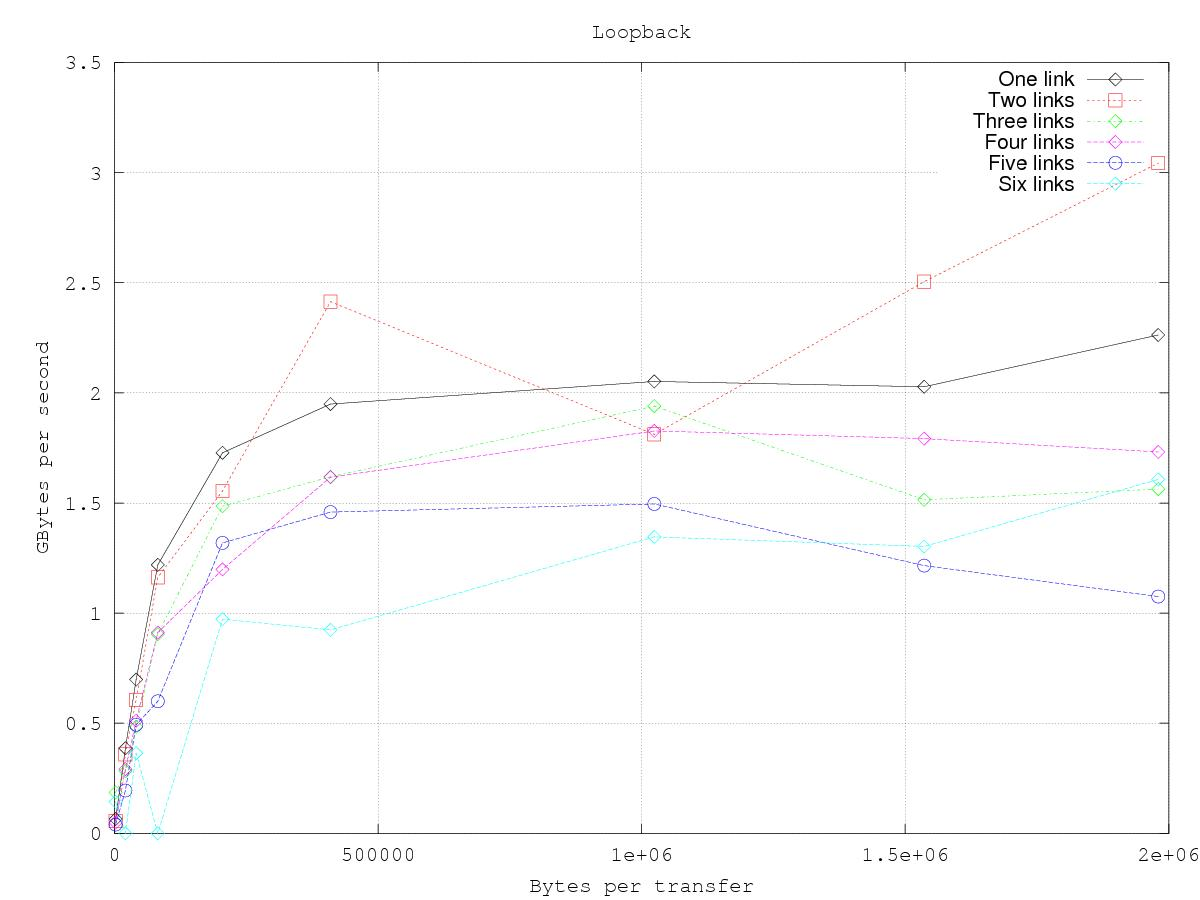
\includegraphics[width=120mm]{optimization/loopback.jpg}
  \caption{Throughput for \ac{bulkio} When Using the Loopback Interface}
  \label{figure:loopbackThroughput}
\end{figure}

Another result derived from the experiment shown in \link {Figure}{figure:loopbackThroughput} is that there is a substantial impact when the number of component pairs transferring data increases.

By following the steps in \link {Section}{section:omniORBConfigurationPipes}, it is possible to achieve higher data rates. \link {Figure}{figure:ldsThroughput} shows the same experiment as that shown in \link {Figure}{figure:loopbackThroughput}, but with omniORB configured for Linux Domain Sockets. As seen in \link {Figure}{figure:ldsThroughput}, sustained data rates on the computer used in this experiment are roughly four times higher when using Linux Domain Sockets compared to using the loopback interface. Even when heavily loaded, the Linux Domain Socket configuration is as fast or faster than the lightly-loaded loopback configuration.

\begin{figure}[H]
  \centering
  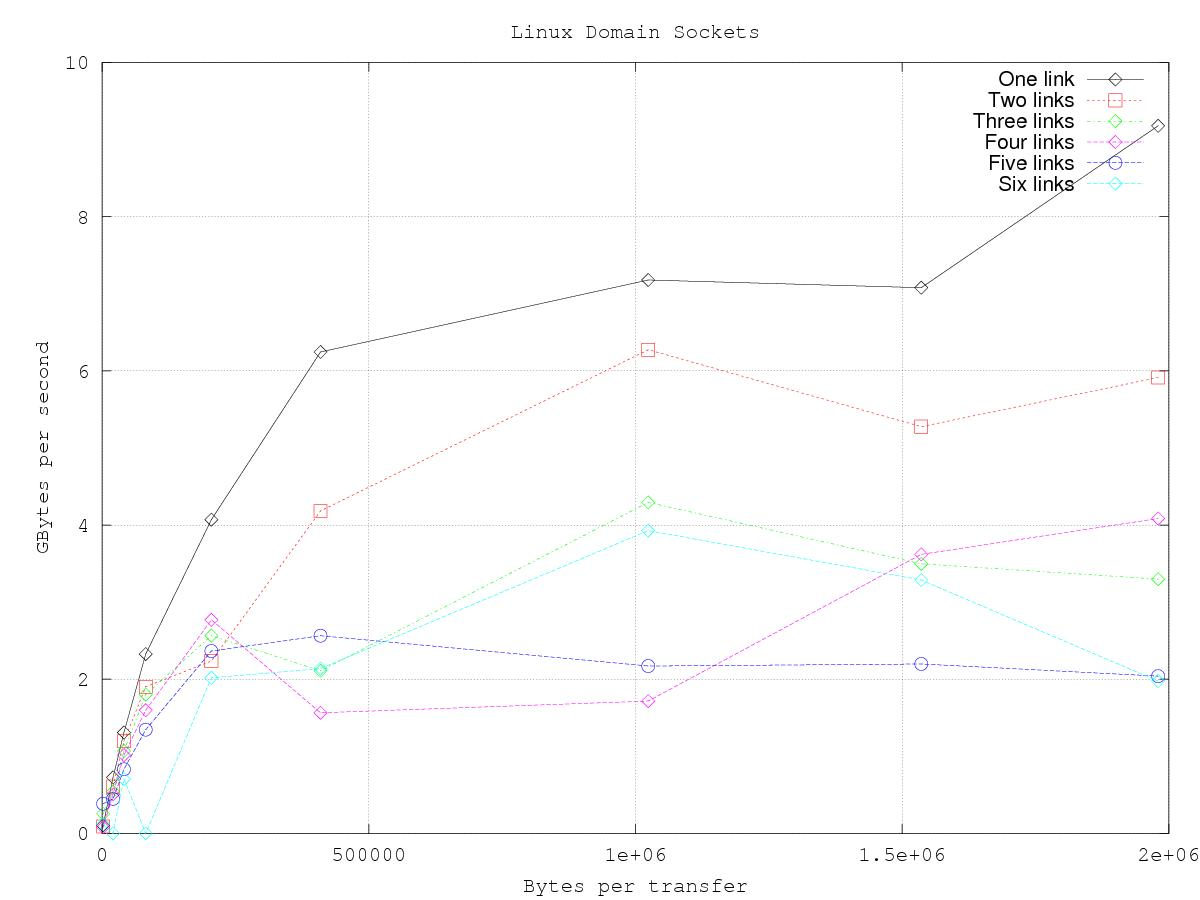
\includegraphics[width=120mm]{optimization/linux_domain_sockets.jpg}
  \caption{Throughput for \ac{bulkio} When Using Linux Domain Sockets}
  \label{figure:ldsThroughput}
\end{figure}

\section{Messaging Latency}

Much like \ac{bulkio}, messaging is subject to performance issues as the transfer size changes. Testing was performed to determine the impact of message size on the latency per message. The size of the message was modified and the latency per message was measured. The average latency was measured for sets of 1000 messages. \link {Figure}{figure:loopLatency} shows the latency results when using the loopback interface and \link {Figure}{figure:ldsLatency} shows the latency when using Linux Domain Sockets. Latency is a function of the size of the message, where the measured latency ranges between 40-150 microseconds and 50-160 microseconds for Linux Domain Sockets and loopback interface, respectively.

\begin{figure}[H]
  \centering
  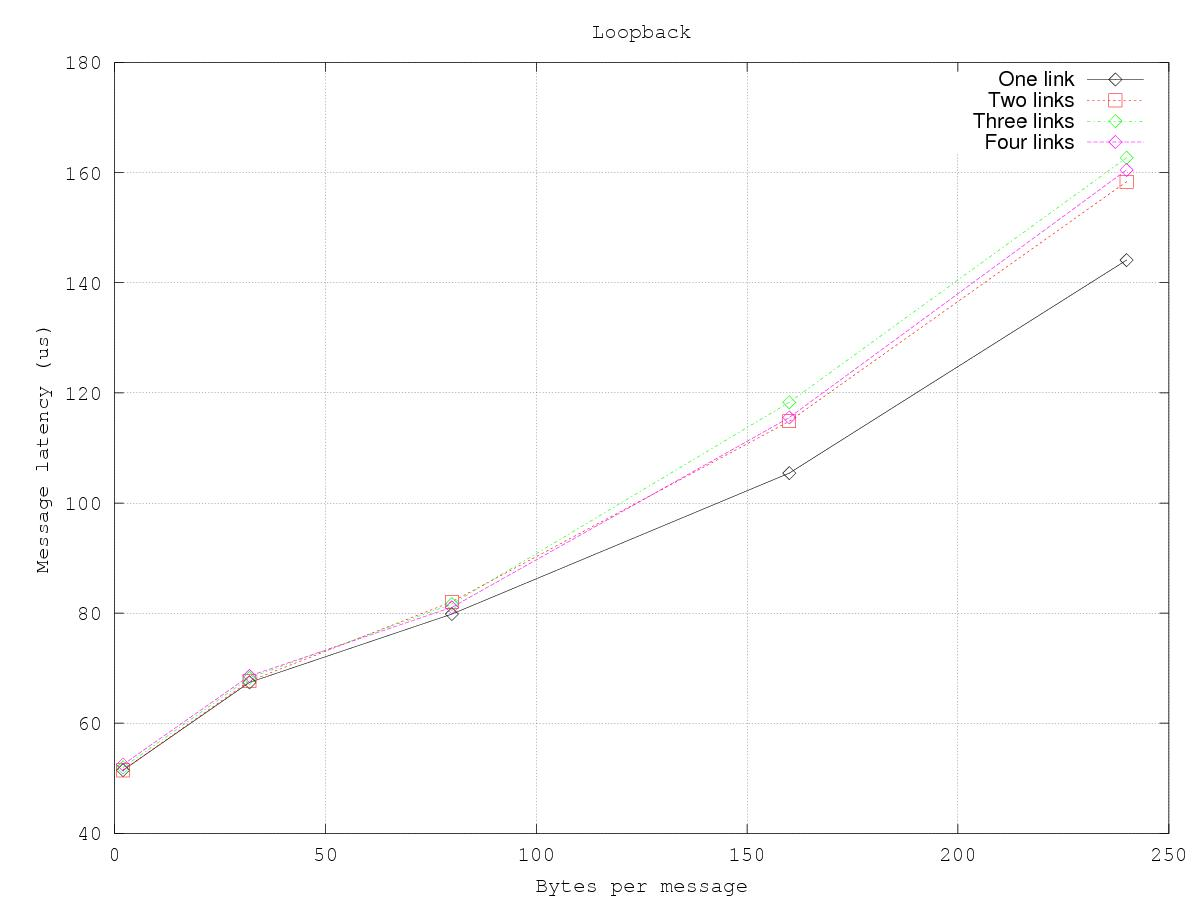
\includegraphics[width=120mm]{optimization/loop_msg.jpg}
  \caption{Message Latency When Using the Loopback Interface}
  \label{figure:loopLatency}
\end{figure}

\begin{figure}[H]
  \centering
  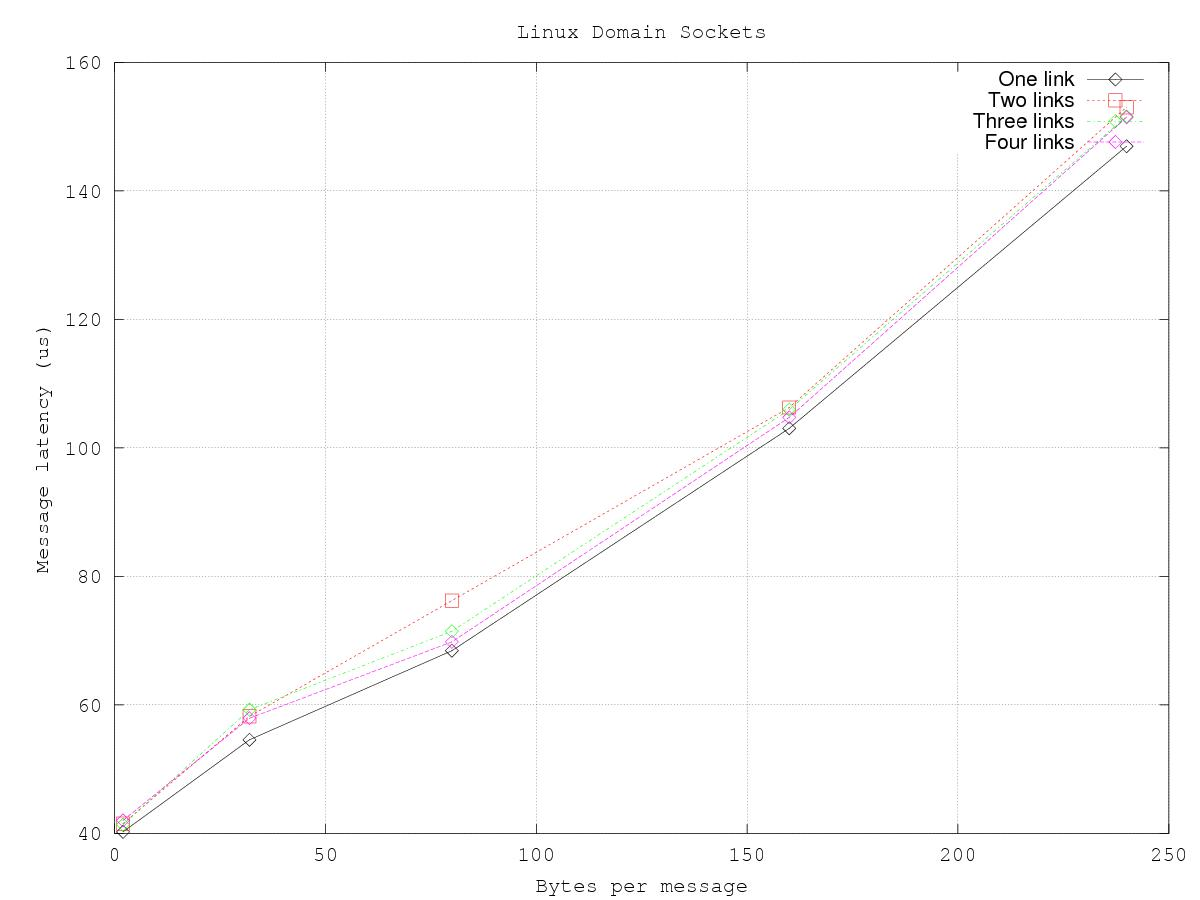
\includegraphics[width=120mm]{optimization/lds_msg.jpg}
  \caption{Message Latency When Using Linux Domain Sockets}
  \label{figure:ldsLatency}
\end{figure}

Note that in \link {Figure}{figure:loopLatency} and \link {Figure}{figure:ldsLatency}, latency is linear as a function of the message size. Furthermore, the number of concurrent messaging components has no discernible impact on the message latency. Finally, the difference shown between Linux Domain Socket performance and loopback interface performance is, while measurable, relatively small.


